\documentclass[tikz,border=10pt]{standalone}
\usepackage{amsmath,amssymb}
\usepackage{tikz}
\usetikzlibrary{arrows,automata,backgrounds,calendar,chains,decorations,decorations.pathreplacing,decorations.text,fit,matrix,mindmap,patterns,petri,plotmarks,positioning,shadows,shapes,shapes.callouts,shapes.geometric,shapes.misc,spy,trees,calc,intersections,tikzmark,arrows.meta}
\usepackage{xcolor}
\usepackage{pgfplots}
\pgfplotsset{compat=1.16}

% Common math macros from the book
\def\x{\mathbf{x}}
\def\y{\mathbf{y}}
\def\z{\mathbf{z}}
\def\A{\mathbf{A}}
\def\b{\mathbf{b}}
\def\c{\mathbf{c}}
\def\w{\mathbf{w}}
\def\v{\mathbf{v}}
\def\u{\mathbf{u}}
\def\e{\mathbf{e}}
\def\zero{\mathbf{0}}
\def\R{\mathbb{R}}
\def\N{\mathbb{N}}
\def\Z{\mathbb{Z}}
\def\Q{\mathbb{Q}}
\def\st{\text{s.t.}}
\def\vect#1{\mathbf{#1}}
\def\xLP{x^{\mathrm{LP}}}
\def\zLP{z^{\mathrm{LP}}}
\def\xIP{x^{\mathrm{IP}}}

% Common node styles from the book
\tikzset{
    main/.style={circle, draw, fill=gray!20, minimum size=1cm, font=\normalsize},
    dot/.style={circle,fill=blue,minimum size=3pt,inner sep=0pt, outer sep=-1pt},
    vertex/.style={circle,fill=black!25,minimum size=20pt,inner sep=0pt},
    edge/.style={draw,-,thick},
    directed edge/.style={draw,->,>=latex,thick},
}

% Additional macros for 3D/coordinate systems
\newcommand{\xhat}{\hat{\x}}
\newcommand{\yhat}{\hat{\y}}
\newcommand{\zhat}{\hat{\z}}
\newcommand{\ihat}{\hat{\imath}}
\newcommand{\jhat}{\hat{\jmath}}
\newcommand{\khat}{\hat{k}}

\begin{document}
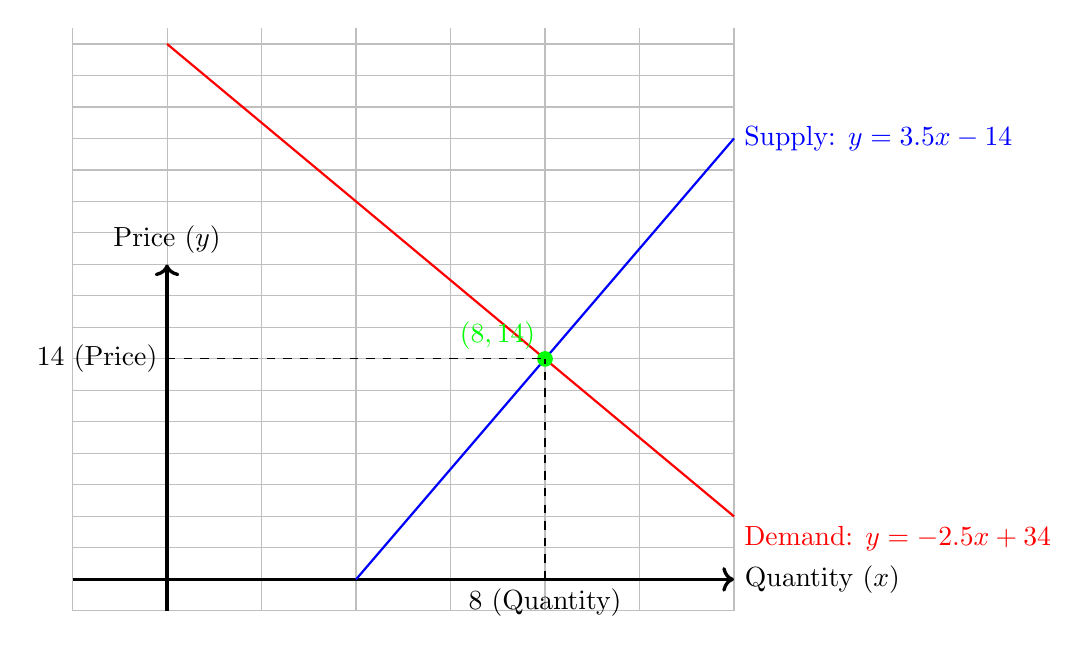
\begin{tikzpicture}[xscale=0.6, yscale=0.2]
    % Grid and axes
    \draw[gray!50, thin, step=2] (-2,-2) grid (12,35);
    \draw[very thick,->] (-2,0) -- (12,0) node[right] {Quantity ($x$)};
    \draw[very thick,->] (0,-2) -- (0,20) node[above] {Price ($y$)};

    % Supply line: y = 3.5x - 14
    \draw[blue, thick] (4,0) -- (12,28) node[anchor=west] {Supply: $y=3.5x-14$};

    % Demand line: y = -2.5x + 34
    \draw[red, thick] (0,34) -- (12,4) node[anchor=north west] {Demand: $y=-2.5x+34$};

    % Intersection point
    \node[green] at (8,14) [circle,fill,inner sep=2pt]{};
    \node[green,anchor=south east] at (8,14) {$(8,14)$};

    % Vertical and horizontal dashed lines to axes
    \draw[dashed] (8,0) -- (8,14);
    \draw[dashed] (0,14) -- (8,14);

    % Labels for equilibrium
    \node[anchor=north] at (8,0) {8 (Quantity)};
    \node[anchor=east] at (0,14) {14 (Price)};
\end{tikzpicture}
\end{document}
